% !TEX root = ../main.tex
\chapter{Related Work} \label{ch:reated_work}

In this chapter, we give an overview of graph based algorithms
for image segmentation.
In \cref{sec:rw_hc} we will discuss hierarchical clustering 
methods.
Watershed methods will be explained in \cref{sec:rw_watershed_methods}
In \cref{sec:energy_based_methods} we will discuss
several energy based methods.
We show prototypical energy functions and
will give a brief overview how those functions can
be optimized.




%\section{Multicut}\label{sec:rw_multicut}
%% !TEX root = ../../main.tex

\section{Multicut}\label{sec:rw_multicut}






\paragraph{Problem Formulation:}














 

%\section{Hierarchical Clustering}\label{sec:rw_hc}
% !TEX root = ../../main.tex
\section{Hierarchical Clustering}\label{sec:rw_hc}

%%%%%%%%%%%%%%%%%%%%%
%dendrogram
%%%%%%%%%%%%%%%%%%%%%%
\begin{figure}
    \centering
    \subfloat[Bottom-Up: Nodes are merged with increasing time]{\label{fig:hc_bottom_up}
        {
            \begin{tikzpicture}[sloped]
                \node (a)    at (-6,0)      {a};
                \node (b)    at (-5,0)      {b};
                \node (c)    at (-4,0)    {c};
                \node (d)    at (-3,0)     {d};
                \node (e)    at (-2,0)       {e};

                \node (ab)   at (-5.5,1)    {};
                \node (cd)   at (-3.5,1)    {};
                \node (cde)  at (-2.75,2)       {};
                \node (all)  at (-4,3)    {};
                
                \node (root) at (-4,4) {root}; 

                \draw (a) |- (ab.center);
                \draw (b) |- (ab.center);
                \draw (c) |- (cd.center);
                \draw (d) |- (cd.center);
                \draw (e) |- (cde.center);
                \draw (cd.center) |- (cde.center);
                \draw (ab.center) |- (all.center);
                \draw (cde.center) |- (all.center);
                \draw (all.center) |- (root.center);

                \draw[->,-triangle 60] (-7,0) -- node[above]{time} (-7,4);
            \end{tikzpicture}
        }
    }\hspace{2cm}
    \subfloat[Top-Down: Nodes are divided with increasing time]{\label{fig:hc_top_down}
        {
            \begin{tikzpicture}[sloped]
                \node (a)    at (-6,0)      {a};
                \node (b)    at (-5,0)      {b};
                \node (c)    at (-4,0)    {c};
                \node (d)    at (-3,0)     {d};
                \node (e)    at (-2,0)       {e};

                \node (ab)   at (-5.5,1)    {};
                \node (de)   at (-2.5,1)    {};
                \node (cde)  at (-3.25,2)       {};
                \node (all)  at (-4,3)    {};
                
                \node (root) at (-4,4) {root}; 

                \draw (a) |- (ab.center);
                \draw (b) |- (ab.center);
                \draw (c) |- (cde.center);
                \draw (d) |- (de.center);
                \draw (e) |- (de.center);        
                \draw (de.center) |- (cde.center);
                \draw (ab.center) |- (all.center);
                \draw (cde.center) |- (all.center);
                \draw (all.center) |- (root.center);

                \draw [->,-triangle 60] (-7,4) -- node[below,align=center]{time} (-7,0);
            \end{tikzpicture}
        }
    }
    \addtocontents{lof}{%
    \vspace{1cm}
    \protect\centerline{%
    \protect\includegraphics[width=.2\linewidth]{fig/thump/dendro.png}
    }%
    }%
    \caption[Bottom-up vs. top-down hierarchical clustering]{
        Describe the difference between both
    }
    \label{fig:hc_bottom_up_top_down}
\end{figure}


Hierarchical clustering techniques have been successfully used
in computer vision since decades \citep{ohlander_1978_cgip,forsyth_2002_book,arbelaez_2006_cvpr,iglesias_2013,morel_1995_book}.

The method  of \citet{ohlander_1978_cgip} is an example for \emph{top-down} clustering,
where all pixel start in one single cluster. Each cluster is recursively divided 
into  more clusters. The method proposed in \cref{ch:cgc} has a strong connection to
\emph{top-down} clustering.
\citet{arbelaez_2006_cvpr} and \citet{iglesias_2013} use the bottom-up approach 
also called \emph{agglomerative clustering}, where 
adjacent nodes in a graph are merged iteratively to create 
a set of nested segmentations.


Such a hierarchy of clusters can be visualized as a dendrogram (see \cref{fig:hc_bottom_up_top_down} ).
The dendrogram can be interpreted as a tree where each node represents a
region in the image.
The leafs in the tree are the atomic units of the image (e.g. pixel,superpixels, supervoxel)
and the root note is the entire scene itself (e.g. the complete image / graph).

There are a few difference between classic unstructured agglomerative clustering
\citep{florek_1951,sokal_1958_science_bulletin,ward_63_jasa}
and agglomerative clustering on graph data structures \citep{arbelaez_2006_cvpr,iglesias_2013,morel_1995_book}, 
e.g. grid-graphs and region adjacency graphs\citep{vlachos_1993_csv}.
While in unstructured hierarchical clustering any pair of observations can be merged,
for graph hierarchical clustering only adjacent nodes / regions can be merged.
In the literature this is also called ``hierarchical clustering with connectivity constraints'' \cite{scikit_learn}.


The main idea behind agglomerative clustering is very simple:

Initially, all observations start in a single cluster. 
Next, cluster which have highest similarities / lowest distances will be merged.
Due to the merging, similarities will change and need to be updated
/ recomputed. Therefore  noisy initial features
will  become more informative .


\begin{table}
\begin{scriptsize}
\begin{tabular}{ |l|l|p{5cm}|}
    \hline 
    Euclidean Distance
        & $||a-b||_2 = \sqrt{\sum{ (a_i-b_i })^2 } $
        & For low dimensional data \\  \hline 
    Squared Euclidean Distance
        & $||a-b||_2^2 = \sum{ (a_i-b_i })^2  $
        & For low dimensions data\\  \hline
    Manhattan Distance
        &  $||a-b||_1 = \sum{ |a_i-b_i |}  $
        & Multi purpose \\  \hline 
    Mahalanobis Distance 
        & $\sqrt{(a-b)S^-1(a-b)^T}$
        & ??? when to use \\  \hline 
    $\mathcal{X}^2$-Distance  
        &  $\frac{1}{2}\sum{  \frac{(a_i-b_i)^2}{a_i+b_i} }$
        & For histograms \\  \hline 
    Earth Mover  Distance          
        &  see \citet{levina_2001_iccv} 
        & For histograms \\  \hline 

\end{tabular}

\end{scriptsize}
\caption{
    An overview of the most common distances measurements and their main properties.
}\label{tab:hc_distance_types}
\end{table}



\begin{table}
\begin{scriptsize}
\begin{tabular}{ |l|l|p{5cm}|}
    \hline
    Average Linkage \citep{sokal_1958_science_bulletin}           
        & $d_{al}(C_a,C_b) = \frac{1}{|C_a||C_b|} \sum _{a \in C_a} \sum_{b \in C_b} d(a,b) $ 
        & \scriptsize Prefers clusters with same variance \cite{sokal_1958_science_bulletin} \\ \hline

    Single Linkage \citep{florek_1951}            
        & $d_{sl}(C_a,C_b) =  \min\{d(a,b) : a \in C_a, b \in C_b\}$ 
        & Nice theoretic properties \citep{hartigan_1981_jjamstat,milligan_1980_psycho}, can lead
          to very irregular shaped clusters \\ \hline
    Complete Linkage \citep{sorensen_1948}         
        & $d_{cl}(C_a,C_b) =  \max\{d(a,b) : a \in C_a, b \in C_b\}$ 
        & Prefers clusters with same diameter \citep{milligan_1980_psycho} \\ \hline
    Centroid Distance         
        & $d_{cd}(C_a,C_b) =  d(\bar{C}_a,\bar{C}_b) $ 
        & Robust w.r.t. outliers \citep{milligan_1980_psycho} \\ \hline
    Wards Minimum Variance \citep{ward_63_jasa}
        & $d_{wmv}(C_a,C_b) = \frac{ d(\bar{C}_a,\bar{C}_b)}{ \frac{1}{|C_a|} + \frac{1}{|C_b|} } $ 
        & Prefers clusters with same size, is sensible to outliers \citep{milligan_1980_psycho} \\ \hline
\end{tabular}

\end{scriptsize}

\caption{
    An overview of the most common cluster distances linkages and their main properties.
}\label{tab:hc_linkage_types}
\end{table}


The definition of a specific distance betweens clusters is very crucial, 
but does strongly depends on the application.
In \cref{tab:hc_distance_types} is a short overview of most common distance
types and in   \cref{tab:hc_linkage_types} is a  brief overview 
of cluster distance linkage types.








\iffalse
\begin{tikzpicture}[scale=  1,every node/.style={minimum size=1cm},on grid]
        
    %slanting: production of a set of n 'laminae' to be piled up. N=number of grids.
    

    %%%%%%%%%%%%%%%%%%%%%%%%%%%%%%%%%%%%%%%%%%%%%%%%%%%%%%%%%%%%%%%
    % 0 bottom layer
    %%%%%%%%%%%%%%%%%%%%%%%%%%%%%%%%%%%%%%%%%%%%%%%%%%%%%%%%%%%%%%%%
        
    \begin{scope}[yshift=0,every node/.append style={yslant=0.5,xslant=-1},yslant=0.5,xslant=-1]
        \draw[-latex,thick] (-0.17,3.21/2) node[right]{\includegraphics[width=4.82cm]{fig/12074/0.png}};
        \draw[black,very thick] (0,0) rectangle (4.81,3.21);
    \end{scope}

    \begin{scope}[yshift=60*1,every node/.append style={yslant=0.5,xslant=-1},yslant=0.5,xslant=-1]
        \draw[-latex,thick] (-0.17,3.21/2) node[right]{\includegraphics[width=4.82cm]{fig/12074/2.png}};
        \draw[black,very thick] (0,0) rectangle (4.81,3.21);
    \end{scope}

    \begin{scope}[yshift=60*2,every node/.append style={yslant=0.5,xslant=-1},yslant=0.5,xslant=-1]
        \draw[-latex,thick] (-0.17,3.21/2) node[right]{\includegraphics[width=4.82cm]{fig/12074/4.png}};
        \draw[black,very thick] (0,0) rectangle (4.81,3.21);
    \end{scope}

    \begin{scope}[yshift=60*3,every node/.append style={yslant=0.5,xslant=-1},yslant=0.5,xslant=-1]
        \draw[-latex,thick] (-0.17,3.21/2) node[right]{\includegraphics[width=4.82cm]{fig/12074/6.png}};
        \draw[black,very thick] (0,0) rectangle (4.81,3.21);
    \end{scope}

    \begin{scope}[yshift=60*4,every node/.append style={yslant=0.5,xslant=-1},yslant=0.5,xslant=-1]
        \draw[-latex,thick] (-0.17,3.21/2) node[right]{\includegraphics[width=4.82cm]{fig/12074/8.png}};
        \draw[black,very thick] (0,0) rectangle (4.81,3.21);
    \end{scope}


    \draw[->,-triangle 60] (-3,0) -- node[above]{time} (-3,4);

    %%%%%%%%%%%%%%%%%%%%%%%%%%%%%%%%%%%%%%%%%%%%%%%%%%%%%%%%%%%%%%%
    % 0 bottom layer
    %%%%%%%%%%%%%%%%%%%%%%%%%%%%%%%%%%%%%%%%%%%%%%%%%%%%%%%%%%%%%%%%
    \draw[-latex,thick] (6.2,2) node[right]{$\mathsf{over-segmentation}$}
         to[out=180,in=90] (4,2);
         
         
         
    %%%%%%%%%%%%%%%%%%%%%%%%%%%%%%%%%%%%%%%%%%%%%%%%%%%%%%%%%%%%%%%
    % 1 layer
    %%%%%%%%%%%%%%%%%%%%%%%%%%%%%%%%%%%%%%%%%%%%%%%%%%%%%%%%%%%%%%%%
    
    \draw[-latex,thick] (6.2,5.5) node[right]{$\mathsf{Region adjacency graph 1}$}
         to[out=180,in=90] (4,5.5);
\end{tikzpicture}
\fi







In the case of graph hierarchical clustering, informative features
can also be attached to the edges of the graph.
Unsupervised edge detectors as gPb \citep{marie_2008_cvpr}  or learned
edge detectors \cite{dollar_2013_iccv}  can be used to boost performance
of agglomerative clustering \citep{arbelaez_2006_cvpr,iglesias_2013}.



\citet{ arbelaez_2006_cvpr} uses $\Omega \in \mathbb{R}^2$ as image domain.
$P_0$ is the inital partition of $\Omega$ and define a
\emph{hierarchical segmentation operator} (HSO) which
assignes a partiton $P_\lambda$ given the inital partiton and
a scale parameter $\lambda$.
Furthermore the follwing properties must be fullfilled for an HSO.  


\begin{align} 
P_{\lambda}  =  P_0 ,\hspace{0.5cm}  \forall \lambda \leq 0  \label{eq:ucm_hco_eq_0} \\ 
\exists \lambda_1 \in \mathbb{R}^+  : P_{\lambda}  =  \{ \Omega \} ,\hspace{0.5cm} \forall \lambda \geq \lambda_1  \label{eq:ucm_hco_eq_1} \\
\lambda < \lambda'  \rightarrow  P_{\lambda} \sqsubseteq   P_{\lambda'} \label{eq:ucm_hco_eq_2}
\end{align}


\Cref{eq:ucm_hco_eq_0} and \cref{eq:ucm_hco_eq_1}  give $\lambda$ a range.
\Cref{eq:ucm_hco_eq_2} ensures that the segmentations are nested.
They define the \emph{salience} of a contour as the scale $\lambda$ where
the contour disappears (see \cref{fig:ucm_visu} )
Thresholding the saliency map will lead to closed contours.
As a consequence, the a complete hierarchical segmentation
generated by a HSO can be encoded in the saliency map.
The formulas and notation of \cref{eq:ucm_hco_eq_0,eq:ucm_hco_eq_1,eq:ucm_hco_eq_3}
has been taken from \citep{ arbelaez_2006_cvpr}.


\citet{iglesias_2013} try to improve segmentation with
the use of agglomerative clustering combined with machine learning.
Their main idea is to combine training data and features at multiple scales
which are generated during the region merging process.
They show that they can outperform the classic approach
of single scale learning.


\begin{figure} 
    \begin{center}
        \subfloat[$K_0$]{ \label{fig:ucm_k0}
            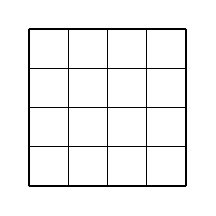
\begin{tikzpicture}
                \draw[step=0.5,black,thin] (0.0,0.0) grid (2,2);
                \draw[step=2,black,thick] (0.0,0.0) grid (2,2);
            \end{tikzpicture}
        }
        \hspace{0.5cm}
        %
        %
        %
        \subfloat[$K_1$]{ \label{fig:ucm_k1}
            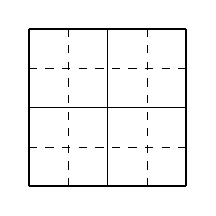
\begin{tikzpicture}
                \draw[step=0.5,black,very thin,dashed] (0.0,0.0) grid (2,2);
                \draw[step=1,black,thin] (0.0,0.0) grid (2,2);
                \draw[step=2,black,thick] (0.0,0.0) grid (2,2);
            \end{tikzpicture}
        }
        \hspace{0.5cm} 
        %
        %
        %
        \subfloat[$K_2$]{\label{fig:ucm_k2}
            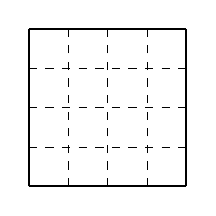
\begin{tikzpicture}
                \draw[step=0.5,black,very thin,dashed] (0.0,0.0) grid (2,2);
                \draw[step=2,black,thick] (0.0,0.0) grid (2,2);
            \end{tikzpicture}
        }
        \hspace{0.5cm}
        %
        %
        %
        \subfloat[$\mathcal{C}(\Upsilon) $]{ \label{fig:ucm_saliency}
            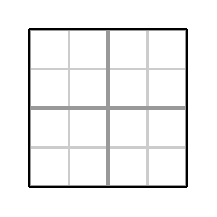
\begin{tikzpicture}
                \draw[step=0.5,black!20,thick] (0.0,0.0) grid (2,2);
                \draw[step=1,  black!40,very thick] (0.0,0.0) grid (2,2);
                 \draw[step=2,black,thick] (0.0,0.0) grid (2,2);
            \end{tikzpicture}
        }
        \hspace{0.5cm}
        %
        %
        %
        \subfloat[$\mathcal{C}(\Upsilon) $]{ \label{fig:ucm_saliency_3d}
            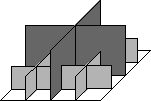
\includegraphics[width=0.2\textwidth]{fig/ucm3d.pdf}
        }
    \end{center}
    \addtocontents{lof}{%
    \vspace{1cm}
    \protect\centerline{%
        \protect\includegraphics[width=.2\linewidth]{fig/thump/ucm.png} 
    }%
    }%
    \caption[Ultra metric contour map saliency]{
        \Cref{fig:ucm_k0} shows the an $4x4$ grid graph which servers as initial segmentation $K_0$.
        \Cref{fig:ucm_k1} shows the segmentation $K_0$ after the contraction of a few edges.
        Contracted edges are showed dashed.
        \Cref{fig:ucm_k2} shows the graph after all edges have been contracted.
        \Cref{fig:ucm_saliency} shows the saliency $\mathcal{C}$ of the contour $\Upsilon$ of the contours.
        In \cref{fig:ucm_saliency_3d} the saliency from \ref{fig:ucm_saliency} as a 3D visualization.
        This figure is very much inspired from a figure showed in \citep{arbelaez_2006_cvpr}.
    }\label{fig:ucm_visu}
\end{figure}




\todo{fredreciks methods for findig cuts in hcluster tree} 

%\section{Watershed Methods}\label{sec:rw_watershed_methods}
% !TEX root = ../../main.tex
\section{Watershed Methods}\label{sec:rw_watershed_methods}

The watershed is a powerful tool for image segmentation and
has been used for this purpose since the work of
\citet{beucher_1979_workshop}.
The literature on watersheds is huge and 
a many definitions and algorithms exist
\citep{vinent_1991_pami,beuchner_1994_waterfall,najman_1994_sp,
roerdink_2000_finf,bertrand_2005_jmiv,cousty_2009_pami,
meyer_2012_corr,meyer_2012_corr2}.
A good overview  of the history of watersheds 
is given in the work of \citet{meyer_2012_corr}.
Recent watershed algorithms are discussed in \citep{meyer_2012_corr2}.

The watershed algorithm can be described with the following  \emph{water flooding} analogy:
A gray-scale  image can be interpreted as height map (see \cref{fig:ws_2d_map}, \cref{fig:ws_2d_map3d}).
The water level is then raised as shown in \crefrange{fig:ws_a}{fig:ws_f}.
A watershed is wherever the water of two adjacent valleys would flow together (see \cref{fig:ws_e}, \cref{fig:ws_f} and \cref{fig:ws_2d_lines}).


An image may be interpreted as a node weighted graph,where the node weights
are given by the pixels gray values.
Watersheds can also be applied to edge weighted graphs, where the nodes are unweighted 
and the edges connecting neighboring nodes encode the height between the pass points of two valleys.
\citet{meyer_2012_corr2} examined the relations between node and edge weighted watersheds, 
and proofed that both can be transformed to each other.





% watersheds illustrated
\begin{figure}[H]
    \centering
    \subfloat[1d Image Data]{ \label{fig:ws_a}
        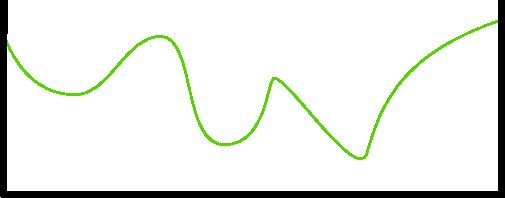
\includegraphics[width=0.25\textwidth]{fig/ws_no_no.pdf}
    }
    \hspace{0.5cm}
    \subfloat[Local minima]{  \label{fig:ws_b}
        \includegraphics[width=0.25\textwidth]{fig/ws_no.pdf}
    }
    \hspace{0.5cm}
    \subfloat[flooding starts]{  \label{fig:ws_c}
        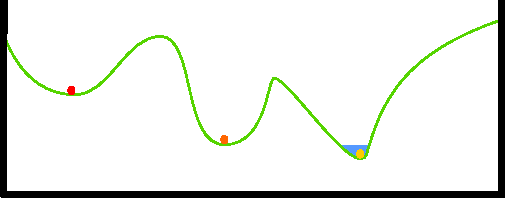
\includegraphics[width=0.25\textwidth]{fig/ws3.pdf}
    }
    \\
    \subfloat[flooding]{  \label{fig:ws_d}
        \includegraphics[width=0.25\textwidth]{fig/ws2.pdf}
    }
    \hspace{0.5cm}
    \subfloat[watershed 1]{  \label{fig:ws_e}
        \includegraphics[width=0.25\textwidth]{fig/ws1.pdf}
    }
    \hspace{0.5cm}
    \subfloat[watershed 2]{ \label{fig:ws_f}
        \includegraphics[width=0.25\textwidth]{fig/ws0.pdf}
    }
    \\ % 2D Watersheds
    \subfloat[$ $]{ \label{fig:ws_2d_map}
        \includegraphics[height=0.26\textwidth]{fig/ws2d0.png}
    }
    \hspace{0.1cm}
    \subfloat[$ $]{ \label{fig:ws_2d_map3d}
        \includegraphics[height=0.26\textwidth]{fig/ws2d1.png} 
    }
    \hspace{0.1cm}
    \subfloat[$ $]{ \label{fig:ws_2d_lines}
        \includegraphics[height=0.26\textwidth]{fig/ws2d2.png}
    }

    \addtocontents{lof}{%
        \vspace{1cm}
        \protect\centerline{%
            \protect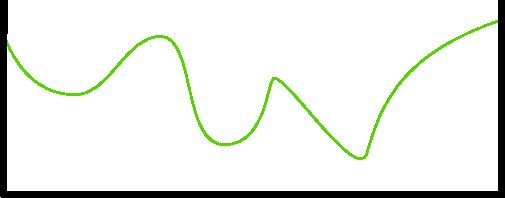
\includegraphics[width=.075\linewidth]{fig/ws_no_no.pdf}  \hspace{0.2cm}
            \protect\includegraphics[width=.075\linewidth]{fig/ws_no.pdf}\hspace{0.2cm}
            \protect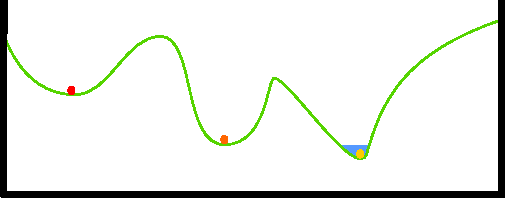
\includegraphics[width=.075\linewidth]{fig/ws3.pdf} 
        }%
        \vspace{0.2cm}
        \protect\centerline{%
            \protect\includegraphics[width=.075\linewidth]{fig/ws2.pdf}  \hspace{0.2cm}
            \protect\includegraphics[width=.075\linewidth]{fig/ws1.pdf} \hspace{0.2cm}
            \protect\includegraphics[width=.075\linewidth]{fig/ws0.pdf}%
        }%
        \vspace{0.2cm}
        \protect\centerline{%
            \protect\includegraphics[height=.075\linewidth]{fig/ws2d0.png}  \hspace{0.2cm}
            \protect\includegraphics[height=.075\linewidth]{fig/ws2d1.png} \hspace{0.2cm}
            \protect\includegraphics[height=.075\linewidth]{fig/ws2d2.png}%
        }%
    }%
    \caption[Illustration of watershed flooding process]{ 
        Illustration of watershed flooding process.
        The water level raises, and the watersheds are at the positions where water from different catchment basins is meeting.
        \Cref{fig:ws_2d_map} to \cref{fig:ws_2d_lines} have been taken from \citep{wiki_watersheds}.
    } \label{fig:watersheds_1d}
\end{figure}







\citet{couprie_2011_pami} proposed the  \emph{power-watershed}  algorithm as a generalization of \citep{ boykov_2001_pami,vinent_1991_pami,najman_1994_sp,roerdink_2000_finf,bertrand_2005_jmiv,sinop_2007_iccv,cousty_2009_pami}.

They define the following model:
\begin{align}\label{eq:power_watershed}
\min_x \sum_{e_{ij} \in E}  w_{ip}^p |x_i-x_j|^q + \sum_{v_i } w_{Fi}^p |x_i|^q + \sum_{v_i } w_{Bi}^p |x_i-1|^q \\
s.t. \hspace{0.35cm} x(F)=1, \hspace{0.5cm} x(B)=0
\end{align}

Where $w_{ip}$ are edge weights and $w_{Fi}^p$ and $w_{Bi}^p$ are unary weights
for foreground and background.

Setting $p$ to 1 will lead to the method proposed by \citet{sinop_2007_iccv}.
\Citet{allene_icv_2010} pointed out, when $p=1$ and $q \rightarrow \infty$, solving
\cref{eq:power_watershed} is equivalent to applying a minimum spanning forest algorithm.
\Cref{tab:power_ws} gives an overview how different choices $p$ and $q$ lead
to different well known segmentation methods, and to the new method, named \emph{power watershed}.

\begin{table}
    \begin{center}
    \begin{tabular}{|l|l|l|l|} \hline
    \backslashbox{$q$}{$p$}        & 0                              & finite & $\infty$              \\ \hline
    $1$           & -      & Graph cuts        & Power watershed           \\ \hline 
    $2$           & L$2$ norm Voronoi           & Random Walker     & Power watershed           \\ \hline 
    $\infty$    & L$1$ norm Voronoi           & L1 norm Voronoi   & Shortest Path Forest      \\ \hline 
    \end{tabular}
    \end{center}
    \caption{ \label{tab:power_ws}
        Power watershed parameterization: Different choices of parameters
        $p$ and $q$ lead to different segmentation methods.
        This table is identical to the table shown in \citet{couprie_2011_pami}.
    }
\end{table}


A drawback of the watershed method is water leaking trough small ``holes'' in the height map/gradient image.
To overcome this weakness, 
\citet{meyer_2002_moprh}  proposed a flooding scheme with viscous mercury-like
liquids.
This idea has been generalized to different viscous fluids in \citep{vachier_2005_jmiv}. 



\citet{straehle_2011_miccai} proposed a watershed-based method for interactive segmentation
of neuro data.
They show how a background prior can be  integrated efficiently into watersheds,
and that such a prior is beneficial for the segmentation of neuro data.
In addition, \citet{straehle_2012_cvpr} proposed an uncertainty estimator for
guided interactive segmentation based on watersheds.

\phantomsection
\label{sec:rw_waterfall}

Edge and node weighted watersheds on graphs can be applied recursively, since
the result of a watershed transformation itself is a more ``coarser'' graph.
This leads to a hierarchy of nested segmentations.
This transformation is called \emph{waterfall transformation} \cite{beuchner_1994_waterfall} and
the hierarchy is called \emph{waterfall hierarchy}.

\Citet{najman_1994_sp} showed, that there is a
strong connection between any hierarchical segmentations
and watersheds.
They prove that there exists a bijection between
the set of ultrametric watersheds \citep{najman_2010_corr} and the set of hierarchical segmentations.

 

%\section{Energy Based Methods}\label{sec:energy_based_methods}
% !TEX root = ../../main.tex
\section{Energy Based Methods}\label{sec:energy_based_methods}

Energy based methods have become very popular recently.

Given a graph $G = (U,V)$ we 
associate  a variable $ x_i \forall \quad u_i \in V$ with any node.
Within this thesis we focus on discrete energy function.
Therefore use discrete variables $x$.
W.l.o.g. we set  $ x_i   \in \{ 0,1,2,\ldots, N_{labels}-1 \} \quad \forall \quad u_i \in V$,
which means that any node has the same number of labels.

An energy function $E(x)$ can be  defined  in the following way:

\begin{equation} \label{eq:gm_energy}
    E(x) = 
    \underbrace{
        \sum_{v \in V} \phi_i(x_i)
    }_{\text{unaries}}
     \quad +  \quad
    \underbrace{
        \sum_{e=(i,j) \in E } \phi_{ij}(x_i,x_j) 
    }_{\text{pairwise terms}}
\end{equation}



Where the \emph{unaries} $\phi_i(x_i)$ encode local costs
for a variable to have certain label.
While the \emph{pairwise terms} $\phi_{ij}(x_i,x_j) $ define the interaction of adjacent nodes.
Often they are used to introduce some smoothness prior
into the model \citep{szeliski_2008_pami,MORE_HERE}.


The vector which yields a minimum value of $E(x)$
is called $x_{\text{optimal}}$.

\begin{equation} \label{eq:gm_argmin}
x_{\text{optimal}} = \argmin_{x}  E(x)
\end{equation}


Before discussing how to optimize such an energy functions,
we will give some concrete examples how $E(X)$ 
can look in real world examples.

\paragraph{Denoising:}


Let $G=(V,E)$ be a grid graph corresponding to
a grayscale image.
Setting $N_{labels}$ to $255$ we can interpret  the variables $x$ directly as
gray values.
Let $I_i$ be the gray value of the pixel associated with variable $x_i$.

\begin{equation} \label{eq:gm_ef_dension}
E(x) = \sum_{v \in V}  (I_i - x_i)^2 + \sum_{e=(i,j) \in E } \lambda (x_i-x_j)^2
\end{equation}

\begin{figure}[H]
    \centering
    \subfloat[Input Image $I$]{ \label{fig:eq:gm_ef_dension_input}
        \includegraphics[width=0.25\textwidth]{fig/houseM-input.png}
    }
    \subfloat[ICM]{ \label{fig:eq:gm_ef_dension_icm}
        \includegraphics[width=0.25\textwidth]{fig/houseM-ICM.png}
    }
    \subfloat[$\alpha$-Expansion]{  \label{fig:eq:gm_ef_dension_ae}
        \includegraphics[width=0.25\textwidth]{fig/houseM-Expansion.png}
    }
    \subfloat[TRWS]{  \label{fig:eq:gm_ef_dension_trws}
        \includegraphics[width=0.25\textwidth]{fig/houseM-TRW-S.png}
    }
    \caption[Energy based truncated denoising]{
        Finding $x_{\text{optimal}} $ for the energy function given
        in \cref{eq:gm_ef_dension} we show result of approximative solvers.
        Using \cref{fig:eq:gm_ef_dension_input} as input (for the black area no unaries 
        are used)
        the following
        results are obtained:
        ICM
         \citep{besag_1986_icm}  (\Cref{fig:eq:gm_ef_dension_icm} ) fails
        to fill the in-painting area. 
        While TRWS
        \citep{kolmogorov_2006_pami_trws}  (\Cref{fig:eq:gm_ef_dension_trws} ) 
        and $\alpha$-Expansion
        \citep{boykov_2001_pami}  (\Cref{fig:eq:gm_ef_dension_ae} ) 
        can fill the in-painting area
        with meaningful values.
        The input image has been taken from \citep{szeliski_2008_pami}.
        The result images have been generated with OpenGM.
    }\label{fig:gm_ef_denoise}
\end{figure}

This model has been proposed by \citep{szeliski_2008_pami} where they proposed a MRF-benchmark.


\paragraph{Truncated Denoising:} 

This model is almost the same as the \emph{Denoising} model defined above,
but the second order term is truncate to $\gamma$ if $(x_i-x_j)^2$ is larger than $\gamma$.
Therefore we do pay only $\gamma$ at strong edges.
This model has also been proposed by \citep{szeliski_2008_pami} within their MRF-benchmark.


\begin{equation} \label{eq:gm_ef_dension_truncated}
E(x) = \sum_{v \in V}  (I_i - x_i)^2 + \sum_{e=(i,j) \in E } \lambda \cdot \min\left( (x_i-x_j)^2, \gamma\right)
\end{equation}

\begin{figure}[H]
    \centering
    \subfloat[Input Image $I$]{ \label{fig:eq:gm_ef_dension_truncated_input}
        \includegraphics[width=0.25\textwidth]{fig/penguin-bar.png}
    }
    \subfloat[ICM]{ \label{fig:eq:gm_ef_dension_truncated_icm}
        \includegraphics[width=0.25\textwidth]{fig/penguin-ICM.png}
    }
    \subfloat[$\alpha$-Expansion]{  \label{fig:eq:gm_ef_dension_truncated_ae}
        \includegraphics[width=0.25\textwidth]{fig/penguin-Expansion.png}
    }
    \subfloat[Trws]{  \label{fig:eq:gm_ef_dension_truncated_trws}
        \includegraphics[width=0.25\textwidth]{fig/penguin-TRW-S.png}
    }
    \caption[Energy based truncated denoising]{
        Finding $x_{\text{optimal}} $ for the energy function given
        in \cref{eq:gm_ef_dension_truncated} we show result of approximative solvers.
        Using \cref{fig:eq:gm_ef_dension_truncated_input} as input (for the black area no unaries 
        are used)
        the following
        results are obtained: ICM \citep{besag_1986_icm}  (\Cref{fig:eq:gm_ef_dension_truncated_icm} ) fails
        to fill the in-painting area. While TRWS \cite{kolmogorov_2006_pami_trws}  (\Cref{fig:eq:gm_ef_dension_truncated_trws} ) 
        and $\alpha$-expansion \cite{boykov_2001_pami}  (\Cref{fig:eq:gm_ef_dension_truncated_ae} ) can fill the in-painting area
        with meaningful values.
        The input image has been taken from \citep{szeliski_2008_pami}.
        The result images have been generated with OpenGM.
    }\label{fig:gm_ef_dension_truncated}
\end{figure}


\paragraph{Submodular Two Class Segmentation:}
    WRITE ME



\paragraph{Multicut Energy Function:}
Removing all unaries from \cref{eq:gm_energy} and 
setting $\phi_{ij}(x_i,x_j) =   \w_e \cdot \delta( x_i \neq x_j )$ 
will lead to the multicut objective (see \cref{sec:rw_multicut} and \cref{ch:cgc}) .

For planar problems  $N_{labels}$ can be set to 4 since any planar map is 4 colorable \citep{appel_1977_4color}.
For non planar problems we need to set $N_{labels}$ to $|V|$.



\begin{align}
E(x)=
    \sum_{ e=(i,j) \in E}
        \w_e \cdot \delta( x_i \neq x_j )
    \label{eq:gm_ef_multicut}
\end{align}


The \emph{max-cut} objective and  the multicut objective
are almost the same, 
but within max-cut problem we have only binary variable $x_i=\{0,1\}$ .

\begin{align}
E(x)=
    \sum_{ e=(i,j) \in E}
        \w_e \cdot \delta( x_i \neq x_j )
    \label{eq:gm_ef_max_cut}
\end{align}




\subsection{Graph Cut Based Methods}

If $N_{labels}=2$ and $\phi_{ij}(x_i,x_j)$ is submodular, 
graph cuts \cite{boykov_2001_pami,kolmogorov_2004_pami} can be applied to find $x_{\text{optimal}}$
in polynomial time.

Graph cut is a optimization algorithm which casts the energy minimizing problem
to the maximum flow / minimum cut problem. Energy function of binary variables which
have a form as 

\begin{equation} \label{eq:gm_graph_cut_energy}
    E(x) = 
    \underbrace{
        \sum_{v \in V} \phi_i(x_i)
    }_{\text{unaries}}
     \quad +  \quad
    \underbrace{
        \sum_{e=(i,j) \in E } \phi_{ij}(x_i,x_j) 
    }_{\text{submodular pairwise terms}}
\end{equation}



where the pairwise energy term of binary variables is submodular can be minimized with
graph cuts. $\phi_{ij}$ is submodular if

\begin{equation} \label{eq:gm_submodular_criterion}
    \phi_{ij}(0,1) + \phi_{ij}(1,0) >  \phi_{ij}(0,0) + \phi_{ij}(1,1)
\end{equation}

To use graph cut, we have to associate each possible solution with a cut on a graph as in
\cref{fig:graph_cut} and ensure that the capacities on the graph match our energy function 
defined in \cref{eq:gm_graph_cut_energy}.
Since the max flow/ min cut problem is defined on a directed graph, we have to construct
a directed graph from the energy function we want to minimize. We add a source and a
sink vertex and connect these terminal vertices with all variable vertices and assign
each edge a non-negative flow capacity. The flow goes from the source vertex to the
sink vertex. The edge capacities are constructed as described in the work of
\citet{kolmogorov_2004_pami}.

\Cref{fig:graph_cut_b} shows how the
construction of the directed weighted graph which associate with the energy function $E(x)$.
\citet{kohli_2007_pami} proposed a method to change some and resolve
the problem efficiently which allows a fast computation
of graph cut min marginal an uncertainties \citep{kohli_2006_eccv,tarlow_2012_cvpr}.


\begin{figure}[H]
\begin{center}
\subfloat[$ $]{\label{fig:graph_cut_a}
    \includegraphics[height=0.3\textwidth]{fig/min_st.pdf}   
}
\hspace{1.5cm}
\subfloat[$ $]{\label{fig:graph_cut_b}
    \includegraphics[height=0.3\textwidth]{fig/min_st_d.pdf}   
}
\end{center}
\caption{
    \Cref{fig:graph_cut_a}: Each variable vertex is connected to the 2 terminal vertices, source s, and
        sink t, the edges between the variables vertices and terminal vertices are
        called t-links, the edges between variables vertices are called n-links. The
        line dotted in green is a cut, separating the variable with state zero from
        those with state one.
    \Cref{fig:graph_cut_b} is a simplification of the construction of the weighted graph.
        A constant term $\beta$ which has to be added to some capacities
        has been omitted for simplicity. 
        Interested readers are refereed to  the work of \citet{kolmogorov_2004_pami}.
}\label{fig:graph_cut}
\end{figure}


Whenever we have a a energy function of binary variables with pairwise potentials which
are non-submodular we cannot use graph cut. QPBO (quadratic pseudo-boolean optimization), 
the work of \citet{rother_2007_cvpr}, 
addresses the problem of minimizing such an energy function as the
following:

\begin{equation} \label{eq:gm_qpbo_energy}
    E(x) = 
    \underbrace{
        \sum_{v \in V} \phi_i(x_i)
    }_{\text{unaries}}
    \quad +  \quad
    \underbrace{
        \sum_{e=(i,j) \in E } \phi^{s}_{ij}(x_i,x_j)
    }_{\text{submodular pairwise terms}}
    \quad +  \quad
    \underbrace{
        \sum_{e=(i,j) \in E } \phi^{\bar{s}}_{ij}(x_i,x_j)
    }_{\text{non-submodular pairwise terms}}
\end{equation}

The basic idea of QPBO is to relax the problem by optimizing an auxiliary graphical
model with twice as much variables as the problem we want to optimize. The
auxiliary problem is constructed in such a way that it is submodular. The
auxiliary problem is constructed as in \cite{rother_2007_cvpr} and optimized with graph cut. 
The output of QPBO
is a partial labeling $x_i \in \{ 0,1, EPT \}$. $EPT$ is interpreted as unknown state. There are several
extension to improve which reduce the number
of variables which have the state $EPT$ .


If the label space is larger than 2, $\alpha$-expansion and $\alpha \beta$-swap \cite{boykov_2001_pami} can be used.
The main idea of $\alpha$-expansionm is to iteratively
solve binary sub-problems, where one only has to decide whether a variable should be
flipped to the state $\alpha$ or keep the current state. The value of $\alpha$ is changed in each iteration.

$\alpha \beta$-swap] is very similar  $\alpha$-expansion.
But this time we have two labels, $\alpha$ and $\beta$. Within each iteration variables
with the state $\alpha$ can be flipped to the state $\beta$ and visa versa. The values of $\alpha$ and $\beta$
are changed after each iteration.

If the binary sub-problems are submodular graph cut can be used, otherwise QPBO.



\subsection{Linear Programming Methods}



An alternative formulation of the multicut objective \cref{eq:multicut_primal,eq:gm_ef_multicut} 
is in terms of binary edge indicator variables.
$\y \in \{0,1\}^{| E |}$:
\begin{align}
\argmin_{\y}
%
\left\{
    \sum_{e=(i,j) \in E} \w \left(e\right) \cdot \y_{e}
\right\}%
%
\;\;\text{s.t.}\;\;\y \in \MC_G.
\label{eq:multicut_dual_a}
\end{align}
%
%
$\text{MC}_G$ is the set of all multicut
constraints \cite{chopra_1993_mp} for graph $G$ forming
the so called \emph{multicut polytope}.
The objective in \cref{eq:multicut_dual_a}
is linear w.r.t. indicator variables $\y_{e}$.

In general,
$\y \in \MC_G$ can be enforced by an exponential number of
constraints \cite{chopra_1993_mp}, but in practice
-- for a given objective function --
a small subset of those are sufficient.
Therefore, a major branch of research has focused 
on cutting plane approaches,
either by solving a relaxation of \eqref{eq:multicut_dual}
by a sequence of linear programs 
\cite{kim_2011_nips,kim_2012_ip,kappes_2013_arxiv,finley_2005_ml}.














To apply linear programming methods to minimize a general discrete energy function, 
the energy functions
needs to be linearized.

To optimize an energy functions as 

\begin{equation} \label{eq:gm_nl_energy}
    E(x) = 
     \sum_{v \in V}
    \underbrace{
        \phi_i(x_i)
    }_{\text{unaries}}
     \quad +  \quad
     \sum_{e=(i,j) \in E } 
    \underbrace{
        \phi_{ij}(x_i,x_j) 
    }_{\text{pairwise terms}}
\end{equation}

we introduce $\mu_{i}^{l}$ as an indicator variable where $\mu_{i}^{l}=1$ indicates $x_i=l$.
In the same manner we use $\mu_{ij}^{l_a l_b}$ to indicate pairwise 
assignments.
The constraints ensure that the indicator variables $\mu_{i}^{l}$ are consistent 
with pairwise indicators $\mu_{ij}^{l_a l_b}$ .

The set of these consistency constraints is 
called \emph{local consistency constraints} \citep{sontag_2010_thesis}.

\begin{align}
    E(\mu) = \sum_{v \in V} \sum_{l=0}^{L_{\text{max}}} \label{eq:gm_lp}
    \mu_{i}^{l} \cdot \phi_{i}( l)
    \quad +  \quad
    %
    \sum_{e \in E} \sum_{l_a=0}^{L_{\text{max}}} \sum_{l_b=0}^{L_{\text{max}}}
    \mu_{ij}^{l_a l_b} \cdot \phi_{ij}( l_a,l_b) \\
    %
    s.t. \quad
    \sum_{l=0}^{L_{\text{max}}} \mu_{i}^{l} = 1 \quad \forall \quad v_i \in V \\
    %
    \sum_{l_b=0}^{L_{\text{max}}} \mu_{ij}^{l_a l_b} = \mu_i 
    \quad \forall \quad e_{ij} \in E, 
    \quad l_a \in \{ 0,1,\ldots,L_{\text{max}} \} \\ 
    %
    \sum_{l_a=0}^{L_{\text{max}}} \mu_{ij}^{l_a l_b} = \mu_j 
    \quad \forall \quad e_{ij} \in E, 
    \quad l_b \in \{ 0,1,\ldots,L_{\text{max}} \} \\ 
    %
    \mu_i^l \geq 0 \quad \forall \quad v_{i} \in V,
    \quad l \in \{ 0,1,\ldots,L_{\text{max}} \}\\
    \mu_{ij}^{l_a l_b} \geq 0 \quad \forall \quad e_{ij} \in E,
    \quad l_a,l_b \in \{ 0,1,\ldots,L_{\text{max}} \}
\end{align}

Solving the LP in \cref{eq:gm_lp} will lead to fractional
solutions since the \emph{local consistency constraints} 
define a polytope which is a relaxation
of the marginal polytope.
In \cref{fig:local_poly} is a visualization of the local
polytope \footnote{
Interested readers are refereed to the doctoral
thesis of  \citet{sontag_2010_thesis} which gives
a great overview and introduction to linear programming
based optimization.
}.

An additional set of constraints, \emph{integer constraint} can be added the LP in \cref{eq:gm_lp}. These constraints turn the LP into an integer LP (I-LP).

\begin{align}
    \mu_i^l \in \{0,1\} \quad \forall \quad v_{i} \in V,
    \quad l \in \{ 0,1,\ldots,L_{\text{max}} \} \label{eq:integral_constraint}
\end{align}

Solving the I-LP yields
global optimal solutions of the energy function defined in 
\cref{eq:gm_nl_energy}.







\begin{figure}[H]
\centering
\includegraphics[width=0.6\textwidth]{fig/frac_vert2.pdf}
\caption{
    A sketch of the local consistency polytope.
    The local polytope is a relaxation
    of the marginal polytope (red dashed lines).
    While the marginal polytope has only integral
    nodes (red nodes , the local polytope 
    will introduce fractional vertices which are shown
    in blue.
    The figure has been taken from \citep{sontag_2010_thesis}
    an has been modified slightly.
    Interested readers are refereed to the doctoral
    thesis of  \citet{sontag_2010_thesis} which gives
    a great overview and introduction to linear programming
    based optimization.
}\label{fig:local_poly}
\end{figure}





 

%\section{MST Methods}\label{sec:rw_mst_methods}
%% !TEX root = ../../main.tex
\section{MST Methods}\label{sec:rw_mst_methods}
Discuss the method from \citet{felzenszwalb_2004_ijcv}.
Discuss the method from \citet{Straehle_k-smallestspanning}. 

%\section{Random Walker}\label{sec:rw_random_walker}
%% !TEX root = ../../main.tex
\section{Random Walker}\label{sec:rw_random_walker}

gready random waler 





%\section{Normalized Cuts}
